\documentclass[a4paper]{article} % set paper size

\usepackage[utf8]{inputenc}
\usepackage {url}
\usepackage[top=2.0cm, bottom=2.0cm, left=2.54cm, right=2.54cm]{geometry} % set margin
\usepackage{amsfonts} % for set names
\usepackage{amsmath} % for equation system
\usepackage{amsthm} % for theorem block
\usepackage{fixltx2e} % for subscript
\usepackage{fancyhdr} % for footer/headline modification
\usepackage{xcolor}
\usepackage{graphicx,float} % for image insertion
\usepackage{multicol} %for text in tow columns

\usepackage{wrapfig} %figure wrapping


\pagestyle{fancyplain} % for footing modification on all pages
\fancyhf{}
%\renewcommand{\headrulewidth}{0pt} % remove decorative lign
\fancyhead[L]{Pauline Maury-Laribiere\\
              Alexandre Devienne}
\fancyhead[R]{MT/EL-BA2 EPFL \\
                \today}
\fancyhead[C]{\textbf{Spring programming project : Microcosmos}}

\fancyfoot[R]{\thepage\ of \pageref{lastpage}}

\begin{document}
\begin{multicols*}{2}
% =====================================================================
\section{Program's architecture}


\begin{figure}[H]
\centering
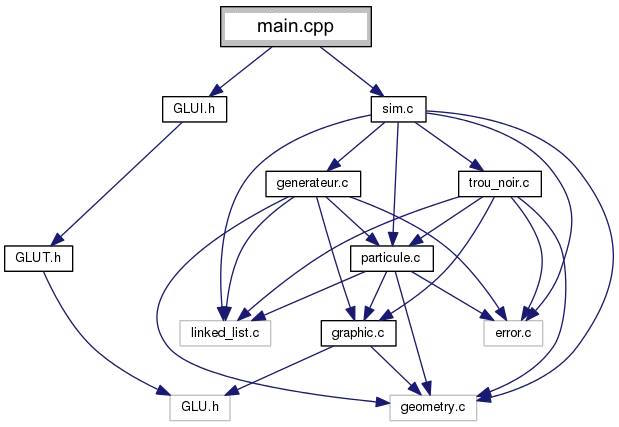
\includegraphics[width=0.45\textwidth]{architecture.jpg}
\caption{Final architecture}
\end{figure}


Compared to the architecture suggested, we added two low level modules, and 2 depencies:
\begin{description}
\item[Module: geometry]
Low level representation of points and vectors and functions to manipulate them (ex: distance between point, norm of a vector)

%This module in included in the modules : \emph{main}, \emph{sim}, \emph{generateur}, \emph{particule}, \emph{trou\_noir}, \emph{graphic}.

\item[Module: linked\_list]
Abstract double linked list data structure.
Some basic dictionary are implemented such as : first, next, add, delete, search.
More complex operation exists such as : sort and calling a function with argument 2 elements, for every possible 2-combinations of elements
(to work out the forces between every particles for example)

%This module in included in the modules : \emph{sim}, \emph{generateur}, \emph{particule}, \emph{trou\_noir}.

\item[Dependency: trou\_noir $\rightarrow$ particule]
This allows \emph{trou\_noir} to call \texttt{part\_applyForceField( void (*forceFieldAt) (POINT p) )}
to apply to all particles the force generated by all black holes.
Plus, to destroy particles too close to a black hole, it can call \texttt{int part\_closestPartOn( POINT p )}
to retrieve a particle's ID to then destroy it with : \texttt{part\_delete( int partID )}

\item[Dependency: generateur $\rightarrow$ particule]
This allows \emph{generateur} to delegate the validity of a generator's argument to \emph{particule}
and to create particle by a simple call of \texttt{part\_create}
\end{description}

Working with these modules ease our work by reducing the amount of redundant code.
It also eased the testing part, as we could validate the correctness of these modules before using them in the project.

% =====================================================================
\section{Data structures}



% =====================================================================
\section{Function called by \emph{main.cpp} from \emph{sim.c}}

\label{lastpage}
\end{multicols*}
\end{document}
